% A LaTeX template for MSc Thesis submissions to 
% Politecnico di Milano (PoliMi) - School of Industrial and Information Engineering
%
% S. Bonetti, A. Gruttadauria, G. Mescolini, A. Zingaro
% e-mail: template-tesi-ingind@polimi.it
%
% Last Revision: October 2021
%
% Copyright 2021 Politecnico di Milano, Italy. NC-BY

\documentclass{Configuration_Files/PoliMi3i_thesis}

%------------------------------------------------------------------------------
%	REQUIRED PACKAGES AND  CONFIGURATIONS
%------------------------------------------------------------------------------

% CONFIGURATIONS
\usepackage{parskip} % For paragraph layout
\usepackage{setspace} % For using single or double spacing
\usepackage{emptypage} % To insert empty pages
\usepackage{multicol} % To write in multiple columns (executive summary)
\setlength\columnsep{15pt} % Column separation in executive summary
\setlength\parindent{0pt} % Indentation
\raggedbottom  

% PACKAGES FOR TITLES
\usepackage{titlesec}
% \titlespacing{\section}{left spacing}{before spacing}{after spacing}
\titlespacing{\section}{0pt}{3.3ex}{2ex}
\titlespacing{\subsection}{0pt}{3.3ex}{1.65ex}
\titlespacing{\subsubsection}{0pt}{3.3ex}{1ex}
\usepackage{color}

% PACKAGES FOR LANGUAGE AND FONT
\usepackage[english]{babel} % The document is in English  
\usepackage[utf8]{inputenc} % UTF8 encoding
\usepackage[T1]{fontenc} % Font encoding
\usepackage[11pt]{moresize} % Big fonts

% PACKAGES FOR IMAGES
\usepackage{graphicx}
\usepackage{transparent} % Enables transparent images
\usepackage{eso-pic} % For the background picture on the title page
\usepackage{subfig} % Numbered and caption subfigures using \subfloat.
\usepackage{tikz} % A package for high-quality hand-made figures.
\usetikzlibrary{}
\graphicspath{{./Images/}} % Directory of the images
\usepackage{caption} % Coloured captions
\usepackage{xcolor} % Coloured captions
\usepackage{amsthm,thmtools,xcolor} % Coloured "Theorem"
\usepackage{float}

% STANDARD MATH PACKAGES
\usepackage{amsmath}
\usepackage{amsthm}
\usepackage{amssymb}
\usepackage{amsfonts}
\usepackage{bm}
\usepackage[overload]{empheq} % For braced-style systems of equations.
\usepackage{fix-cm} % To override original LaTeX restrictions on sizes

% PACKAGES FOR TABLES
\usepackage{tabularx}
\usepackage{longtable} % Tables that can span several pages
\usepackage{colortbl}

% PACKAGES FOR ALGORITHMS (PSEUDO-CODE)
\usepackage{algorithm}
\usepackage{algorithmic}

% PACKAGES FOR REFERENCES & BIBLIOGRAPHY
\usepackage[colorlinks=true,linkcolor=black,anchorcolor=black,citecolor=black,filecolor=black,menucolor=black,runcolor=black,urlcolor=black]{hyperref} % Adds clickable links at references
\usepackage{cleveref}
% I CHANGED BELOW TWO LINES
\bibliographystyle{unsrtnat}
\usepackage[numbers,sort&compress]{natbib}

% OTHER PACKAGES
\usepackage{pdfpages} % To include a pdf file
\usepackage{afterpage}
\usepackage{lipsum} % DUMMY PACKAGE
\usepackage{fancyhdr} % For the headers
\fancyhf{}

% Input of configuration file. Do not change config.tex file unless you really know what you are doing. 
% Define blue color typical of polimi
\definecolor{bluepoli}{cmyk}{0.4,0.1,0,0.4}

% Custom theorem environments
\declaretheoremstyle[
  headfont=\color{bluepoli}\normalfont\bfseries,
  bodyfont=\color{black}\normalfont\itshape,
]{colored}

% Set-up caption colors
\captionsetup[figure]{labelfont={color=bluepoli}} % Set colour of the captions
\captionsetup[table]{labelfont={color=bluepoli}} % Set colour of the captions
\captionsetup[algorithm]{labelfont={color=bluepoli}} % Set colour of the captions

\theoremstyle{colored}
\newtheorem{theorem}{Theorem}[chapter]
\newtheorem{proposition}{Proposition}[chapter]

% Enhances the features of the standard "table" and "tabular" environments.
\newcommand\T{\rule{0pt}{2.6ex}}
\newcommand\B{\rule[-1.2ex]{0pt}{0pt}}

% Pseudo-code algorithm descriptions.
\newcounter{algsubstate}
\renewcommand{\thealgsubstate}{\alph{algsubstate}}
\newenvironment{algsubstates}
  {\setcounter{algsubstate}{0}%
   \renewcommand{\STATE}{%
     \stepcounter{algsubstate}%
     \Statex {\small\thealgsubstate:}\space}}
  {}

% New font size
\newcommand\numfontsize{\@setfontsize\Huge{200}{60}}

% Title format: chapter
\titleformat{\chapter}[hang]{
\fontsize{50}{20}\selectfont\bfseries\filright}{\textcolor{bluepoli} \thechapter\hsp\hspace{2mm}\textcolor{bluepoli}{|   }\hsp}{0pt}{\huge\bfseries \textcolor{bluepoli}
}

% Title format: section
\titleformat{\section}
{\color{bluepoli}\normalfont\Large\bfseries}
{\color{bluepoli}\thesection.}{1em}{}

% Title format: subsection
\titleformat{\subsection}
{\color{bluepoli}\normalfont\large\bfseries}
{\color{bluepoli}\thesubsection.}{1em}{}

% Title format: subsubsection
\titleformat{\subsubsection}
{\color{bluepoli}\normalfont\large\bfseries}
{\color{bluepoli}\thesubsubsection.}{1em}{}

% Shortening for setting no horizontal-spacing
\newcommand{\hsp}{\hspace{0pt}}

\makeatletter
% Renewcommand: cleardoublepage including the background pic
\renewcommand*\cleardoublepage{%
  \clearpage\if@twoside\ifodd\c@page\else
  \null
  \AddToShipoutPicture*{\BackgroundPic}
  \thispagestyle{empty}%
  \newpage
  \if@twocolumn\hbox{}\newpage\fi\fi\fi}
\makeatother

%For correctly numbering algorithms
\numberwithin{algorithm}{chapter}

%----------------------------------------------------------------------------
%	NEW COMMANDS DEFINED
%----------------------------------------------------------------------------

% EXAMPLES OF NEW COMMANDS
\newcommand{\bea}{\begin{eqnarray}} % Shortcut for equation arrays
\newcommand{\eea}{\end{eqnarray}}
\newcommand{\e}[1]{\times 10^{#1}}  % Powers of 10 notation

%----------------------------------------------------------------------------
%	ADD YOUR PACKAGES (be careful of package interaction)
%----------------------------------------------------------------------------

%----------------------------------------------------------------------------
%	ADD YOUR DEFINITIONS AND COMMANDS (be careful of existing commands)
%----------------------------------------------------------------------------

%----------------------------------------------------------------------------
%	BEGIN OF YOUR DOCUMENT
%----------------------------------------------------------------------------

\begin{document}

\fancypagestyle{plain}{%
\fancyhf{} % Clear all header and footer fields
\fancyhead[RO,RE]{\thepage} %RO=right odd, RE=right even
\renewcommand{\headrulewidth}{0pt}
\renewcommand{\footrulewidth}{0pt}}

%----------------------------------------------------------------------------
%	TITLE PAGE
%----------------------------------------------------------------------------

\pagestyle{empty} % No page numbers
\frontmatter % Use roman page numbering style (i, ii, iii, iv...) for the preamble pages

\puttitle{
	title=Title Related to Microservices, % Title of the thesis
	name=Ömer Esas, % Author Name and Surname
	course=Computer Science and Engineering - Ingegneria Informatica, % Study Programme (in Italian)
	ID  = 917254,  % Student ID number (numero di matricola)
	advisor= Prof. Elisabetta Di Nitto, % Supervisor name
	coadvisor={Name Surname, Name Surname}, % Co-Supervisor name, remove this line if there is none
	academicyear={2021-22},  % Academic Year
} % These info will be put into your Title page 

%----------------------------------------------------------------------------
%	PREAMBLE PAGES: ABSTRACT (inglese e italiano), EXECUTIVE SUMMARY
%----------------------------------------------------------------------------
\startpreamble
\setcounter{page}{1} % Set page counter to 1

% ABSTRACT IN ENGLISH
\chapter*{Abstract} 
Here goes the Abstract in English of your thesis followed by a list of keywords.
\\
\\
\textbf{Keywords:} here, the keywords, of your thesis % Keywords

% ABSTRACT IN ITALIAN
\chapter*{Abstract in lingua italiana}
Qui va l'Abstract in lingua italiana della tesi seguito dalla lista di parole chiave.
\\
\\
\textbf{Parole chiave:} qui, vanno, le parole chiave, della tesi % Keywords (italian)

%----------------------------------------------------------------------------
%	LIST OF CONTENTS/FIGURES/TABLES/SYMBOLS
%----------------------------------------------------------------------------

% TABLE OF CONTENTS
\thispagestyle{empty}
\tableofcontents % Table of contents 
\thispagestyle{empty}
\cleardoublepage

%-------------------------------------------------------------------------
%	THESIS MAIN TEXT
%-------------------------------------------------------------------------
% In the main text of your thesis you can write the chapters in two different ways:
%
%(1) As presented in this template you can write:
%    \chapter{Title of the chapter}
%    *body of the chapter*
%
%(2) You can write your chapter in a separated .tex file and then include it in the main file with the following command:
%    \chapter{Title of the chapter}
%    \input{chapter_file.tex}
%
% Especially for long thesis, we recommend you the second option.

\addtocontents{toc}{\vspace{2em}} % Add a gap in the Contents, for aesthetics
\mainmatter % Begin numeric (1,2,3...) page numbering

% --------------------------------------------------------------------------
% NUMBERED CHAPTERS % Regular chapters following
% --------------------------------------------------------------------------
\chapter{Introduction}

\chapter{State of the Art}
\label{ch:art}%

\section{Microservice Architecture}
\label{sec:ms_arch}

Although the microservice architecture style has already been a de-facto standard for some large tech companies, and is being embraced by numerous firms in the industry, because of the novelty of the architecture, not all developers and architects in the tech industry and researchers in the academia are aware of what it means and which paradigms it advertises.
Microservice architecture is, not in the least meaning of the word, vastly different from the traditional way of building a web application, namely the monolithic architecture.
Hence, it is a valuable effort to define microservice architecture, what it is about and describe features and trends from which this rather unorthodox architecture emerged.
\\
Most importantly, microservice architecture is, as the name suggests, a software architecture.
There are numerous and slightly different definitions based on the particular discipline of software engineering for what a software architecture is.
However, a very simple yet powerful definition is, a (software) architecture is a representation of significant design decisions that shape a system, where significant is measured by the cost of change \cite{booch}. 
In the case for microservice architecture, the most signification design decision is, splitting the system into small, autonomous services that work together.
Focusing on each element of this design decision will bring about more clarity about the architecture.
\\
First, the microservice architecture divide the system into parts, as other architectural styles do, based on various point of views of the system.
Single Responsibility Principle, one of the famous SOLID principles of software engineering, promotes the idea that every module, class or a function in a computer program should have responsibility over a single part of that program's functionality, and it should encapsulate that part \cite{srp}.
The microservice architecture takes that idea to the extreme and encourages developing independent microservices that tackles just one business functionality.
Unlike a monolithic application, the system is not layered as database, back-end and front-end, or more generally, data, logic and UX layers, but consists of microservices that are created around business capabilities, as displayed in Figure~\ref{fig:monovsmicro}.

\begin{figure}[H]
    \centering
    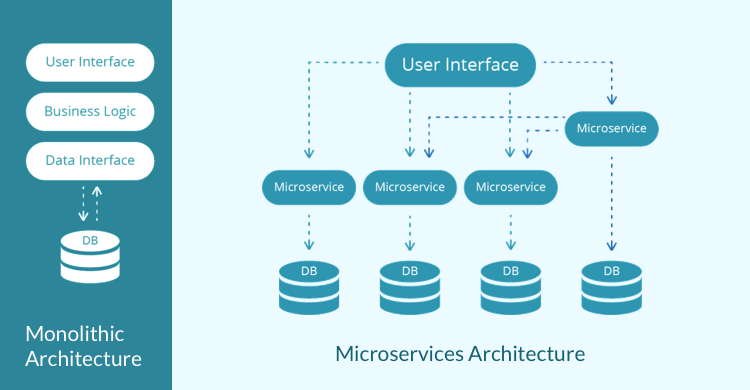
\includegraphics[width=0.75\textwidth]{myImages/monolithic-vs-microservices.png}
    \caption{Monolithic vs Microservice Architecture}
    \label{fig:monovsmicro}
\end{figure}

Second, the microservice architecture advocates for those services to be small.
It is not easy and in some cases inaccurate (e.g, in terms of LOC) to give an estimate of the magnitude of a service, however, a rule of thumb to keep in mind is, microservices should be small enough and not smaller \cite{newman}.
Each service should focus on one business functionality and do it well.
\\
Third, and the last major aspect that defines the microservice architecture is autonomy.
Each service in the microservice architecture is a separate entity, even to the degree that they are mostly designed, developed and deployed by separate teams.
Each team has staff that can together carry out full range of skills required for development, such as database, UX and project management.
\\
At this point, in order to summarize the mentioned major aspects of the microservice architecture and make the architecture more concrete by adding a bit more detail about the implementation, it is a good opportunity to take a look at the definition of the microservice architecture given by an influential software engineer in the field.
According to M. Fowler, the microservice architecture is, "in short, an approach to developing a single application as a suite of small services, each running in its own process and communicating with lightweight mechanisms, often an HTTP resource API.
These services are built around business capabilities and independently deployable by fully automated deployment machinery.
There is a bare minimum of centralized management of these services, which may be written in different programming languages and use different data storage technologies." \cite{microdef}.
In the next section, each characteristic of the microservice architecture is explained in more detail.

\subsection{General Characteristics}
\label{subsec:chars}

\begin{itemize}
    \item Each microservice is developed by a small, cross-functional team.
    The team decides which programming language(s) and technology stack to choose to implement the microservice, and has their own CI/CD tools for testing, release and deployment.
    Each microservice is considered not just a project, but a product, and the development teams are responsible also for the deployment and production process of their microservice, in the Amazon's notion of "you build it, you run it" \cite{youbuild}.
    
    \item Each microservice is a light-weight component that is independently deployable. In case of a change in a particular library, systems that have multiple libraries in a single process like a monolithic architecture has to redeploy entire application. Instead, in a same scenario, having multiple services facilitates redeploying only the changed service. Moreover, this kind of ease in deployment enables the system to be more fault-tolerant and scalable in a more dynamic way, as illustrated Figure~\ref{fig:scalability}.
    
    \begin{figure}[H]
    \centering
    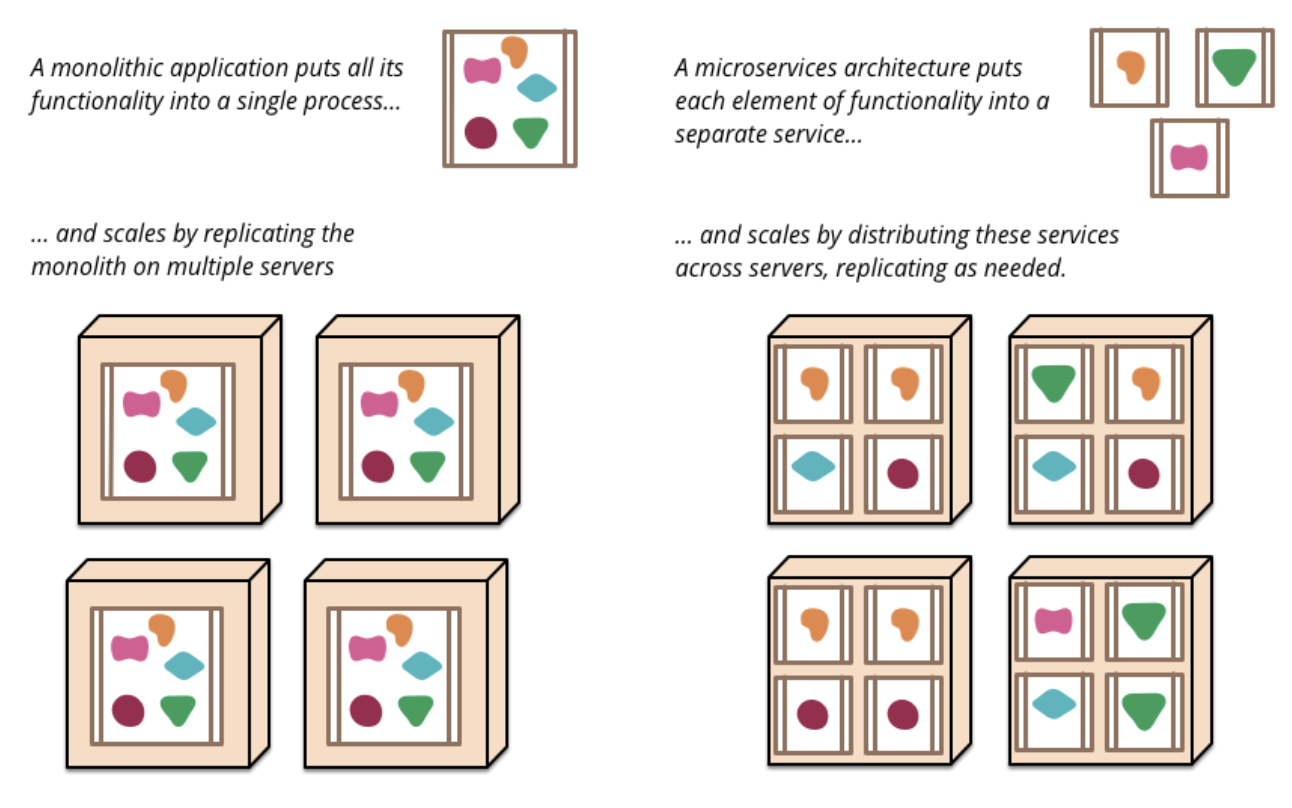
\includegraphics[width=0.75\textwidth]{myImages/scalable.png}
    \caption{Scalability in Monolithic vs Microservice Apps}
    \label{fig:scalability}
\end{figure}

    \item Microservices communicate with each other by means of network calls, using well-defined APIs, and simple protocols like REST over HTTP. While some other architectures incorporate smart (and heavy-weight) messaging mechanisms, such as Enterprise Service Buses (ESB) that can do routing, transformation, choreography and some business logic, the microservice architecture opt for simple communication infrastructure that can do basic routing of messages. In short, they have smart endpoints and dumb pipes.

    \item Each microservice is a loosely-coupled business unit, that is responsible for a single part of the business capability.
    Each model of a microservice is designed on a Bounded Context, which is a part of Domain Driven Design technique \cite{boundedcontext}. Conceptual model of the real world entities are decentralized, meaning that the representation (name) and modeling (attributes) of same real world entities are distinct. Figure~\ref{fig:micromodel} illustrates an example bounded context design and highlights the different representation of the same entity in different microservices.
    
    \begin{figure}[H]
    \centering
    \subfloat[Same Concept as Different Model Entities in Different Microservices\label{fig:micromodel1}]{
        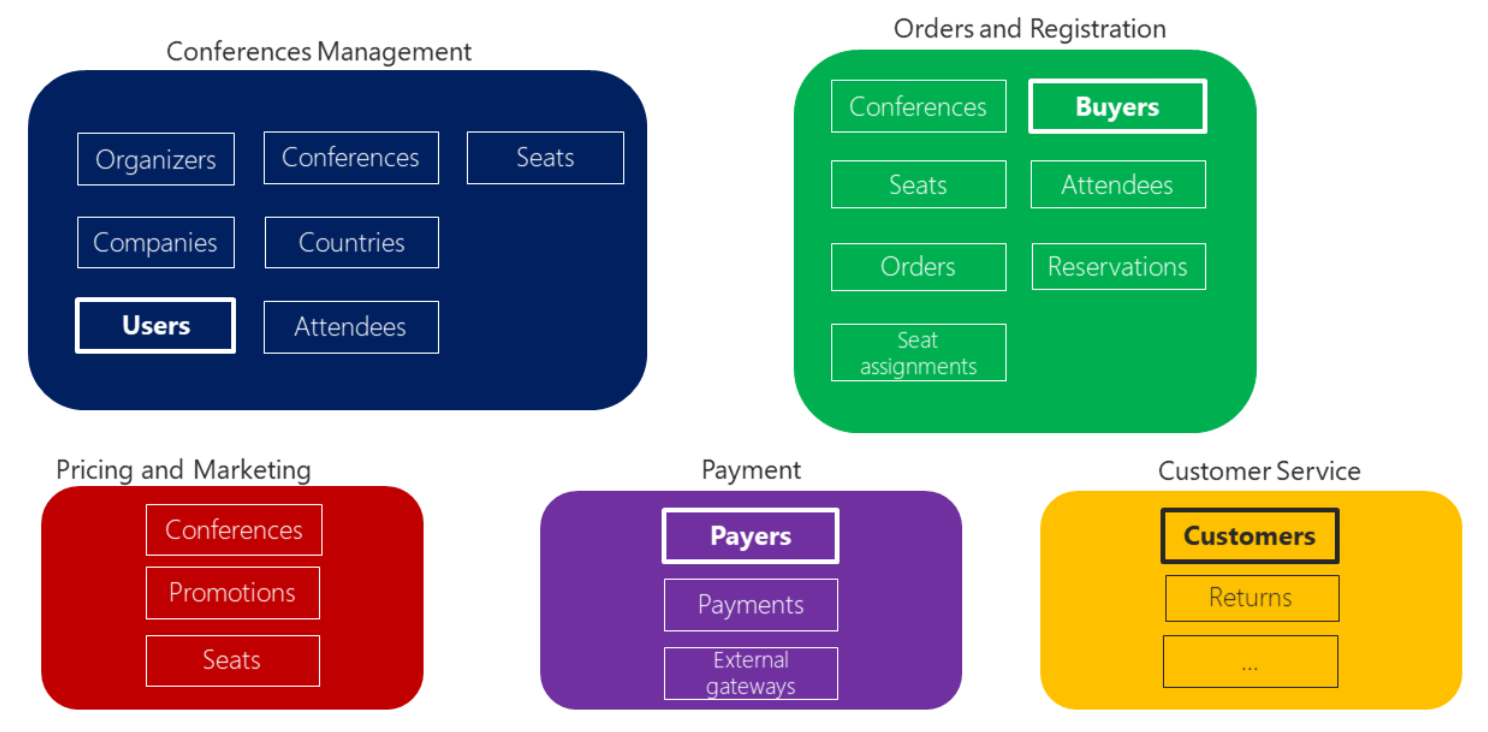
\includegraphics[scale=0.4]{myImages/micromodel1.png}
    }
    \quad
    \subfloat[Decomposing Traditional Data Models\label{fig:micromodel2}]{
        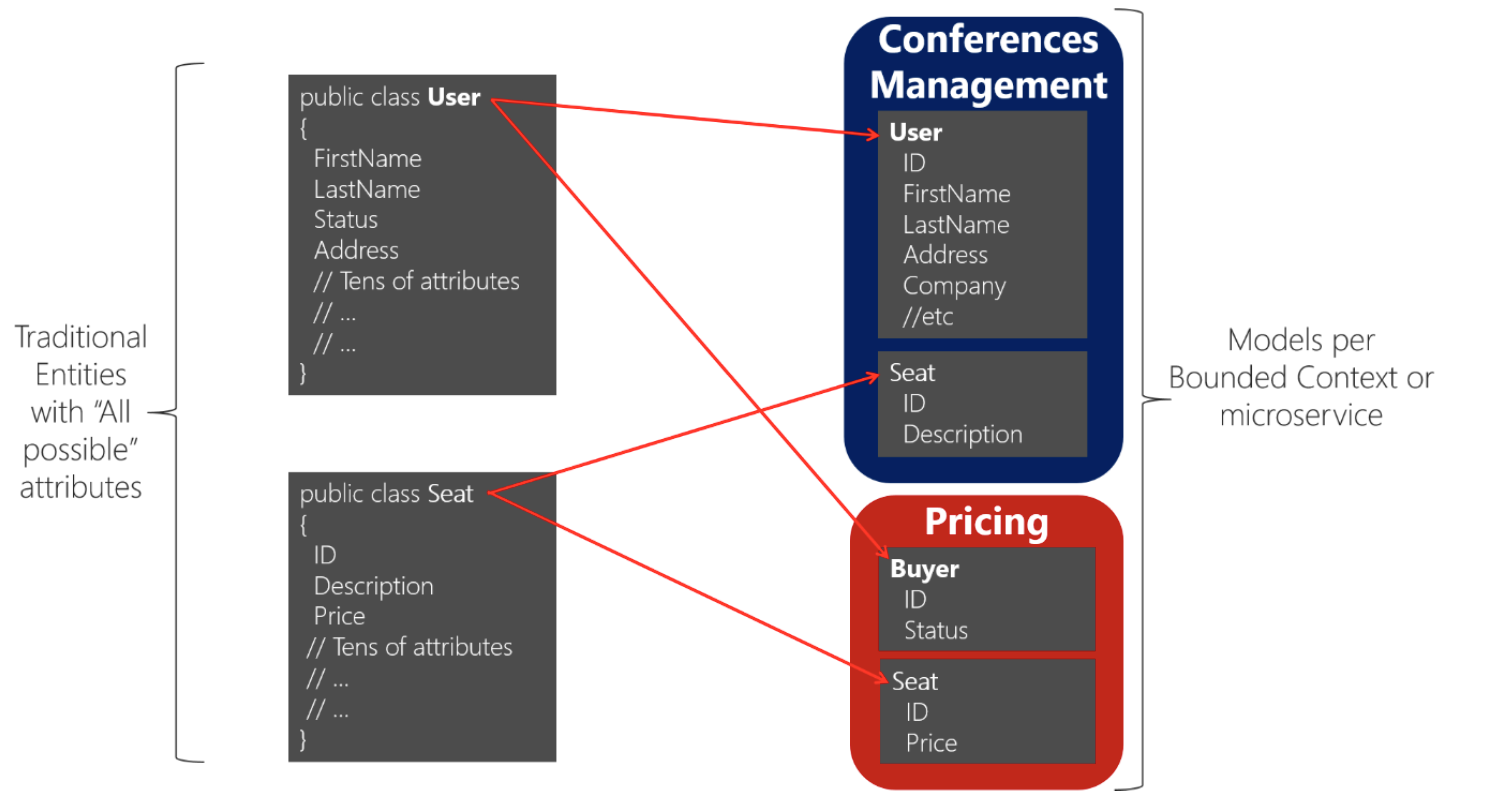
\includegraphics[scale=0.45]{myImages/micromodel2.png}
    }
    \caption{A Microservices Design Using Bound Context Model per Microservice}
    \label{fig:micromodel}
\end{figure}

    \item Just like the decentralized modeling, the persistence layer of the whole application is decentralized, in other words, each microservice and associated team is responsible for managing their own data. The team decides on which kind of database (SQL, NoSQL, graph, columnar, etc) they make use of, taking into consideration their own models and needs.

\end{itemize}

\subsection{Differences from Service Oriented Architecture}
\label{subsec:diff}

The profound idea of microservice architecture, which proposes splitting a system into loosely-coupled, reusable, specialized components is not new.
In the late 90's, Service Oriented Architecture (SOA) emerged as an enterprise-wide approach to software development of components that takes advantage of reusable software components, or services.
Similar to microservice architecture, each service is designed to execute business functions.
\\
Although the two architectures look quite identical at the first glance, they take different different stands on the solutions of common problems in software architecture and therefore there are substantial differences between the two.
Listing the distinctions under three categories will help explain the difference.

\begin{itemize}
    \item Scope: SOA in general relates to enterprise-wide service exposure, while the microservice architecture has an application scope.
    The services are designed using common standards across development teams, aiming at re-usability and sharing of components, resources and data. On the other hand, microservices architecture embraces more relaxed governance approach, giving development teams more freedom of choice.
    Foregoing potential re-usability of code and data, microservice architecture prefers de-coupling of teams and services.
    
    \item Granularity: Having "re-usability across enterprise-wide system" in mind results in services that are fewer in number and larger in size in SOA. Each service typically handles more business functionality than microservices do. As for the persistence, SOA has a single data storage layer which is shared by all services, while each microservice has its own persistence mechanism, if needed for its specific business functionality. Although this results in data duplication in microservice architectures, it enables each microservice to be independent business unit in general \cite{soa_granularity}.
    Moreover, with respect to fine-grained microservices, coarse-grained services in SOA causes time-consuming deployment and less scalability.
    
    \item Communication: SOA makes use of ESB concept, which can handle, in addition to the communication between services using multiple protocols (RESTful API, SOAP, AMQP, MSMQ), management and configuration of services and even some business logic if needed \cite{soa_comm}.
    Having multiple capabilities like these can solve difficult integration problems in large scale systems, however, can possess the danger of single point of failure.
    In addition, the services across the enterprise frequently make synchronous calls, which can lead to latency issues and impact performance.
    To keep things simple, within an application scope, the microservice architecture prefers less elaborate and straightforward  messaging protocols such as HTTP, REST and Thrift.
    To provide communication and data synchronization across microservices, asynchronous communication models like event sourcing and pub/sub model are preferred.
\end{itemize}

\section{Design Patterns and Anti-Patterns in Microservices}
\label{sec:patterns}

Since its introduction by Netflix and discussions at workshops and software architecture conferences, the microservices architecture has gained quite a lot of popularity.
As the architecture is adopted more and more as time goes, legacy systems have been migrated and new projects have been developed utilizing the microservice architecture.
By sharing the experience after successful projects, similar to the evolution of design patterns in other paradigms, reusable solutions to commonly occurring problems have been identified and consequently design patterns in the microservice architecture showed up.
On the flip side, there has also been sub-optimal solutions during this period, resulting from several factors, some of which might be lack of experience, misunderstanding of the microservice architecture or just old habits from SOA.
In the same manner as design pattern, the anti-patterns of the microservice architecture has been identified by researcher and experienced engineers.
In the next two sections, the design patterns and anti-patterns are explored.

\subsection{Design Patterns}
\label{subsec:designpattern}

\subsubsection{API Gateway}
\label{subsubsec:api_gateway}

API gateway acts as a single entry point for all clients as well as an edge service for exposing microservices to the outside world as managed APIs.
It sounds like a reverse proxy, but also has additional responsibilities like simple load-balancing, authentication, authorization, failure handling, auditing, protocol translations, and routing. An API Gateway should always be a highly-available and performant component, since it is the entry point to the entire system, as illustrated in Figure~\ref{fig:api_gateway}.

\begin{figure}[H]
    \centering
    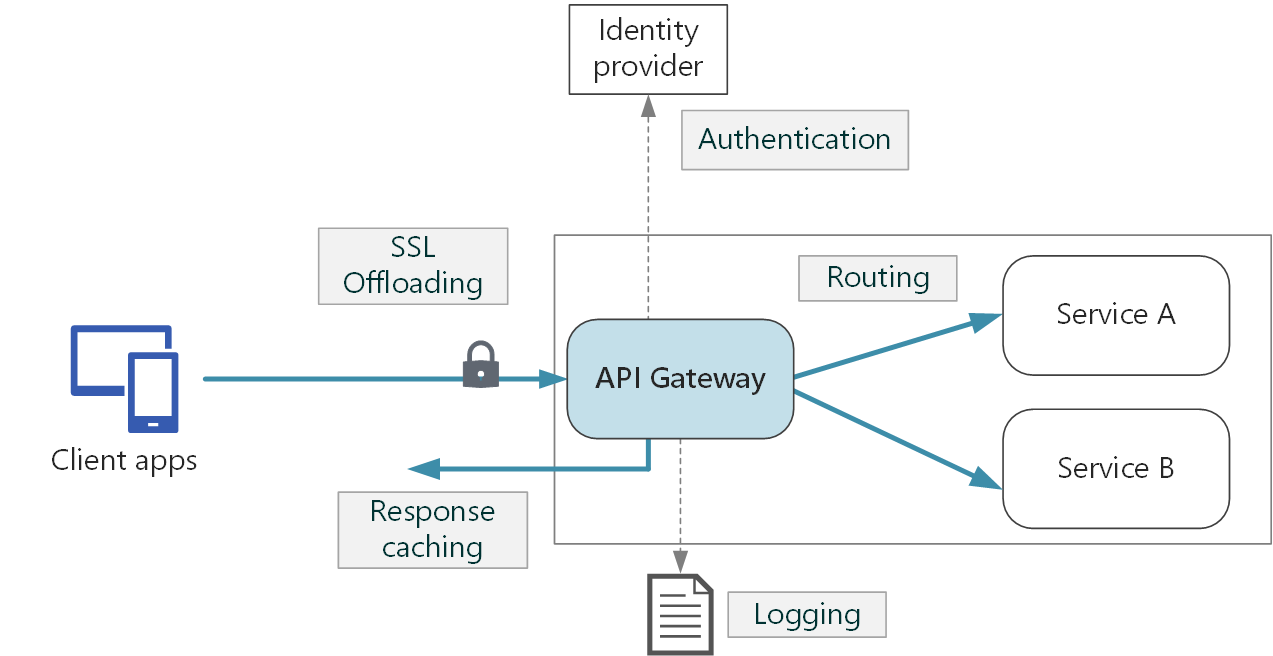
\includegraphics[width=0.75\textwidth]{myImages/api_gateway.png}
    \caption{An example of an API Gateway pattern}
    \label{fig:api_gateway}
\end{figure}

The most common duties of an API gateway include:

\begin{itemize}
    \item Gateway Aggregation: Aggregate multiple client requests (usually HTTP requests) targeting multiple internal microservices into a single client request, reducing chattiness and latency between consumers and services.
    
    \item Gateway Offloading: Enable individual microservices to offload their shared service functionality to the API gateway level.
    Such cross-cutting functionalities include authentication, authorization, service discovery, fault tolerance mechanisms, QoS, load balancing, logging, analytics etc.
    
    \item Gateway Routing (layer 7 routing, usually HTTP requests): Route requests to the endpoints of internal microservices using a single endpoint, so that consumers don’t need to manage many separate endpoints.
\end{itemize}

Developers can choose from implementing their own API gateway, using an existing API gateway solution such as Kong or Express-Gateway, or in case of cloud deployment, choose from products such as Google Apigee, AWS API Gateway or Azure API Gateway.

\subsubsection{Service Mesh with Sidecar}
\label{subsubsec:service_mesh}

A service mesh is a configurable , low-latency infrastructure layer that is designed to tackle high volume of network-based inter-process communication among  application infrastructure services through APIs.
Service mesh pattern is in general implemented as an array of lightweight network proxies called sidecar, without needing the application to be aware of proxies \cite{li2019service}. The sidecar proxies in each service instance handles inter-process communication, monitoring and many other concerns.
Some aspects provided by this helper infrastructure include resiliency (fault tolerance, load balancing), service discovery, routing, observability, security, access control, communication protocol support and alike.
\\
The service mesh pattern is divided into two parts, namely, the control part and the data part, commonly referred as the control plane and the data plane. The control plane generates routing tables and deploy routing configuration to the proxies in the data plane. The actual forwarding of the network traffic is done by the proxies in the data plane, and for this reason, the data plane is also said to be the forwarding plane. Figure~\ref{fig:service_mesh} shows the diagram of an application with service mesh pattern, with the distinction of the control and data planes.

\begin{figure}[H]
    \centering
    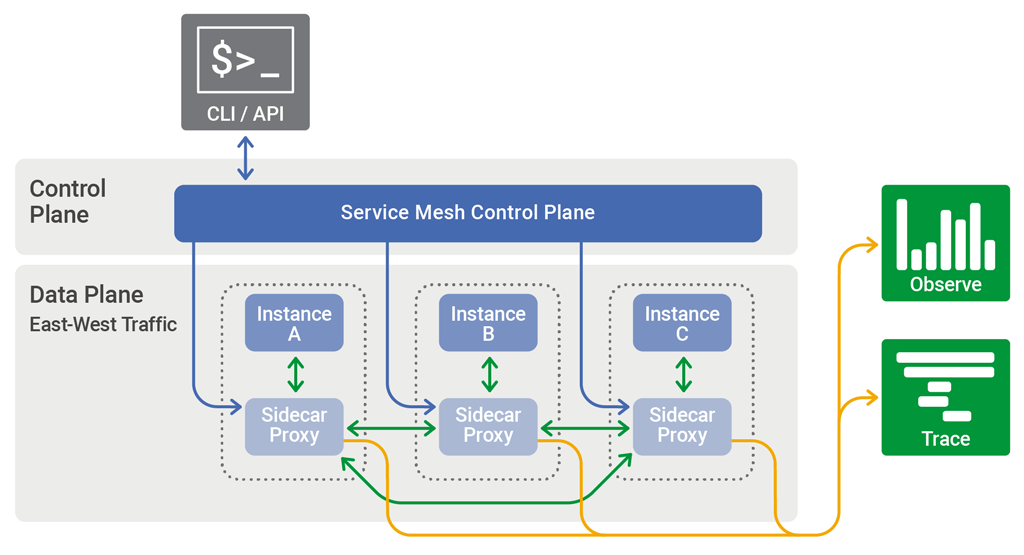
\includegraphics[width=0.75\textwidth]{myImages/service_mesh.png}
    \caption{An Application Architecture utilizing Service Mesh with Sidecar Proxy }
    \label{fig:service_mesh}
\end{figure}

Some of the advantages of making use of a service mesh are:

\begin{itemize}
    \item Logic Decoupling: Decoupling of network communications from microservice business logic code allows developers to focus on the business capabilities.
    
    \item Routing: Primitive routing capabilities, but no routing logic related to the business functionality of the service.
    
    \item Resiliency for inter-service communications: Circuit-breaking, retries and timeouts, fault injection, fault handling, load balancing and fail-over. 
    
    \item Service Discovery: Discovery of service endpoints through a dedicated service registry.
    
    \item Observability: Metrics, monitoring, distributed logging, distributed tracing.
    
    \item Security: Transport level security (TLS) and key management.
    
    \item Access Control: Simple blacklist and whitelist based access control.
    
    \item Deployment: Native support for containers, Docker and Kubernetes. Inter-service communication protocols: HTTP1.x, HTTP2, gRPC.
\end{itemize}

Implementations of the service mesh pattern include products such as Istio, Linkerd and Consul Connect.

\subsubsection{Service Registry and Discovery}
\label{subsubsec:srd}

In order for services to communicate, they expose a remote API at a particular location, specified by host and port number.
However, their number of service instances and locations change dynamically.
Scaling of services are done thanks to virtualization/containerization technologies and virtual machines and containers are usually assigned dynamic IP addresses.
For a service client to get a service, it needs to know the location of that particular service and this is done through service registry and discovery pattern.
When making a request, the client (of a service, it can be API gateway or another service), consults, directly or indirectly, to a service registry that keeps the up-to-date addresses of all service instances.
The clients of the service registry need to know the location(s) of the service registry instances.
Service registry instances must be deployed on fixed and well known IP addresses.
Clients are configured with those IP addresses.
Although clients should cache data provided by the service registry, if the service registry fails that data will eventually become out of date. 
Consequently, the service registry must be highly available.

\begin{itemize}
    \item Service Registry: Service instances register themselves or a third party registers the service.
    A service registry might invoke a service instance’s health check API to verify that it is able to handle requests. Systems that provide service registry include middlewares such as Netflix Eureka, Apache Zookeeper; and service meshes such as Consul and Etcd. Some other systems such as Kubernetes, Marathon and AWS ELB have implicit service registry.
    
    \item Client-side Service Discovery: Query (of service registry) logic is built into the client.
    Spring Boot and Spring Cloud provides client-side service discovery, which is implemented by Netflix OSS (Open Source Software) components: service registry Eureka and HTTP client Ribbon that queries Eureka registry.
    
    \item Server-side Service Discovery: The client makes the request via a router that runs on a well known location.
    The router queries a service registry, which might be built into the router, and forwards the request to an available service instance.
    As an example, AWS Elastic Load Balancer acts as a router that load balances both external and internal traffic and also acts as a service registry.
    EC2 instances are registered with the ELB either explicitly via an API call or automatically as part of an auto-scaling group.
    Some clustering solutions such as Kubernetes and Marathon run a proxy (“service” in Kubernetes terminology) on each host that functions as a server-side discovery router.
    In order to access a service, a client connects to the local proxy using the port assigned to that service.
    The proxy then forwards the request to a service instance (or to controller such as ingress-nginx) running somewhere in the cluster.

\end{itemize}

\subsubsection{Backends For Frontends}
\label{subsubsec:bff}

Instead of using one common backend service for multiple clients, there are separate deployments of the same service with different configurations or implementations that can meet different UI requirements of different clients.
Each one is provides an API for its client.
Because each backend is specific to one interface, it can be optimized for that interface.
Each interface team has autonomy to control their own backend and doesn't rely on a centralized backend development team.

\subsubsection{Asynchronous Messaging}
\label{subsubsec:async_msg}

The distributed nature of microservices requires messaging mechanisms, ideally in a loosely-coupled manner.
The synchronous messaging results in tight run-time coupling, that is, both the client and the service need to be available during the whole messaging period.
To solve these issues and improve scalability, asynchronous messaging mechanisms are widely used in microservices architecture.
Solutions typically include light-weight event buses and message brokers.
Although an extra layer adds complexity, event buses and message brokers decrease run-time coupling by buffering messages, in other words, allowing the recipient to process messages when it becomes available.
Moreover, topics and content filtering can be used to create subsets of messages, delivered only to the interested parties.
With the help of built-in mechanisms of message brokers, different asynchronous messaging styles such as request/response, notification and publish/subscribe can be achieved.
Figure~\ref{fig:rabbitmq} illustrates an example diagram that includes RabbitMQ as a message broker, providing the publish/subscribe messaging manner.

\begin{figure}[H]
    \centering
    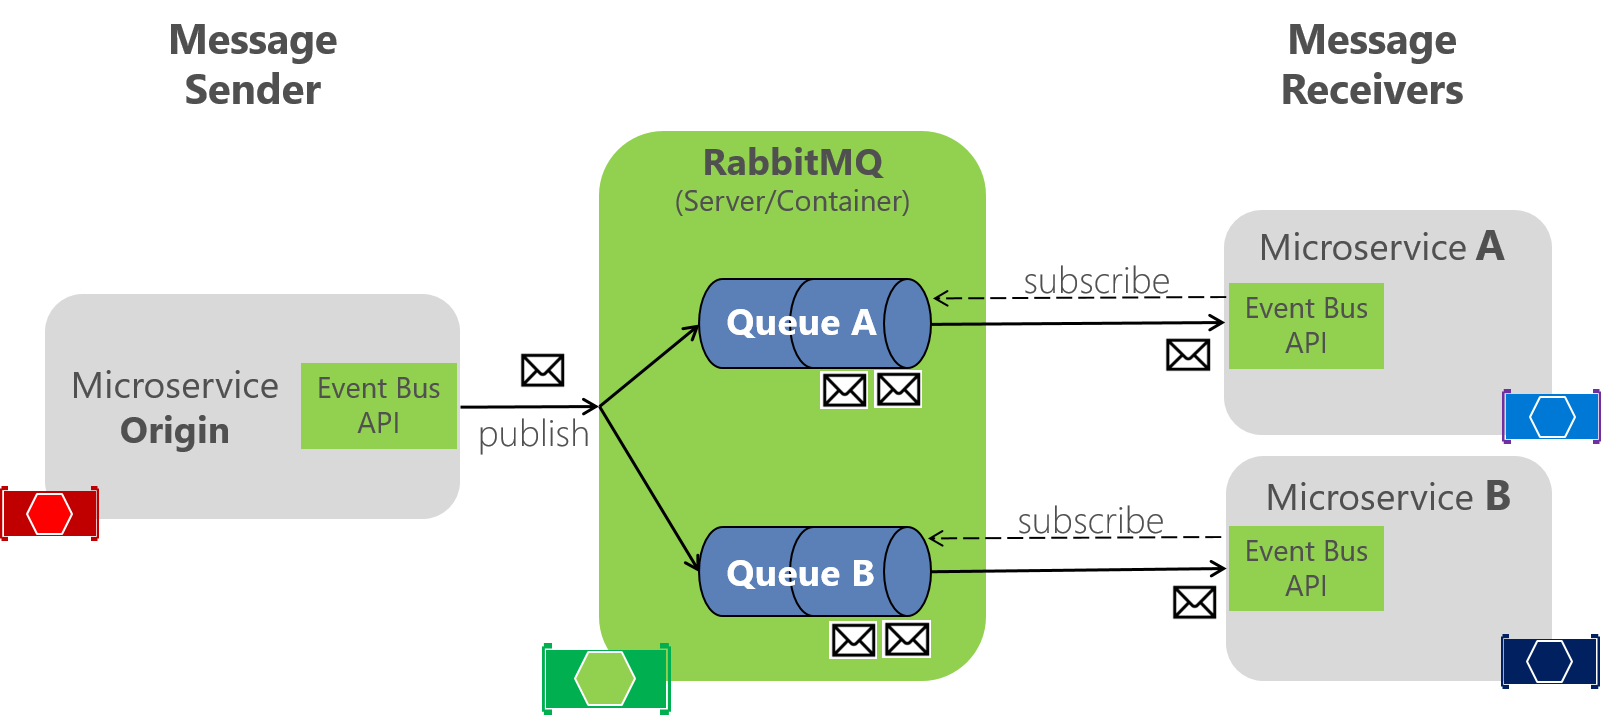
\includegraphics[width=0.75\textwidth]{myImages/rabbitmq.png}
    \caption{RabbitMQ Message Broker with Pub/Sub Mechanism}
    \label{fig:rabbitmq}
\end{figure}

Implementations of message brokers include RabbitMQ and Apache Kafka.
The Key-Value store Redis can also be used as a message broker.
In addition, cloud providers offers message brokers and event buses with different capabilities, such as AWS SNS, AWS SQS, AWS Eventbridge, Azure Event Bus, Google Cloud Tasks and Google Cloud Pub/Sub.

\subsubsection{Database per Service}
\label{subsubsec:dps}

For the sake of loose-coupled services, each service’s persistent data is private to that service and accessible only via its API.
Even though keeping private tables or schema per service facilitates private data, having separate database instances per service also enables the deployment and scaling of services and the teams to be more independent.
By this means, each service can use the type of database that is best suited to its needs.
For example, a service that does text searches could use ElasticSearch, while
another service that manipulates a social graph could use Neo4j.
Although having a separate database server per service is aligned with loose coupling idea, it increases complexity in terms of implementation of transactions that span multiple services, since many NoSQL databases do not support conventional atomic distributed transactions, such as 2-Phase Commit \cite{twopc}.

\subsubsection{Saga}
\label{subsubsec:saga}

In order to solve the issue of implementing business transactions across multiple services, each multi-service transaction is implemented as a sequence of local transactions, which is called a saga.
If a local transaction fails because it violates a business rule then the saga executes a series of compensating transactions that undo the changes that were made by the preceding local transactions.
The two ways of implementing a saga pattern are:

\begin{itemize}
    \item Choreography-based Saga: A transaction is first targeted to a particular service (“order” service receives “POST/orders” request).
    The service completes local transaction with its own database and emits an event to the event bus or a particular event channel (“order created” event in “order events” or a common channel).
    The service that subscribed to that kind of event sees the emitted event and does its own logic and local transaction to its own database and emits another event for any service that listens for that kind of event.
    If all steps are successful, the last service will let the first service know by emitting an event.
    Otherwise, if a failure occurs in a step, the service that could not get its job done (in terms of logic or infrastructure) fires a failure event for the previous step, so the services that have worked before this step can sequentially perform rollbacks.
    A diagram of choreography-based saga pattern is illustrated in Figure~\ref{fig:saga}.
    
    \begin{figure}[H]
    \centering
    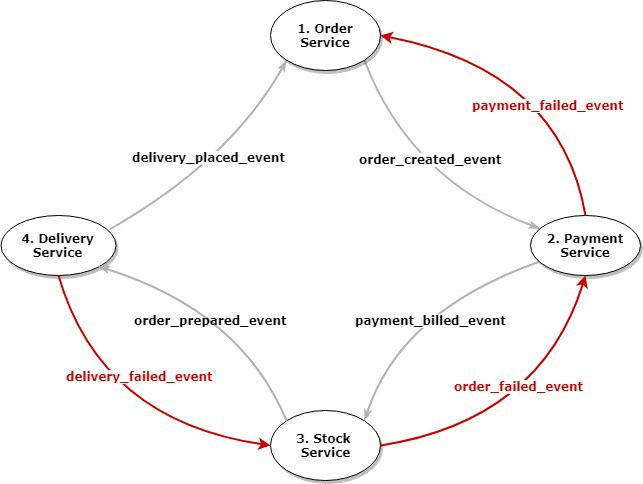
\includegraphics[width=0.65\textwidth]{myImages/saga.jpeg}
    \caption{Choreography-based Saga Pattern}
    \label{fig:saga}
    \end{figure}
    
    \item Orchestration-based Saga: In this approach, unlike the above method, there is an orchestrator that manages the entire transaction.
    When a transaction order that is related to multiple services comes to the service (again, such as “POST/orders”), the service sends a command to the orchestrator.
    The orchestrator starts calling services to be called (directly or indirectly) and after a successful response, it calls the next one. Upon an answer that tells about a failure, the orchestrator then starts sending rollback messages to the previous services.
    With respect to the choreography approach, this method brings about scalability and single point of failure issues.

\end{itemize}

\subsubsection{API Composition}
\label{subsubsec:api_comp}

A simple way to implement queries that spans multiple services is API composition pattern
API composer service can take the query, then starts querying individual services that are related to the main query, join the responses and format the main query result to the client.
However, some queries would result in inefficient, in-memory joins of large datasets.

\subsubsection{Command Query Responsibility Segregation (CQRS)}
\label{subsubsec:cqrs}

Another way to respond to a query that covers numerous services is Command Query Segregation Pattern.
A service is wrapped around a view database that is a read-only replica that fulfils the query responsibility of the application.
The service keeps the database up-to-date by subscribing to domain events, published by the service that owns the data.
As the name suggests, separate services are responsible for the query (read) and command (write and any other logic) parts of the application.
Although it comes with potential complexity, code duplication and eventually consistent view nature, it supports multiple de-normalized views that are scalable and performant.

\subsubsection{Event Sourcing}
\label{subsubsec:event_sourcing}

A service typically needs to update its data and send/publish messages.
For example, a service that participates in a saga needs to atomically update the database and sends messages/events.
If the database transaction commits messages must be sent.
Conversely, if the database rolls back, the messages must not be sent.
In addition, messages must be sent to the message broker in the order they were sent by the service.
This ordering must be preserved across multiple service instances that update the same aggregate.
\\
A good solution to this problem is to use event sourcing pattern.
Event sourcing persists the state of a business entity such as Order or a Customer as a sequence of state-changing events.
Whenever the state of a business entity changes, a new event is fired from the respective microservice, and stored in a database named as the event store, which can be an ACID-compliant database, a time-series database or a database server specifically implemented for event sourcing pattern, such as EventStore.
The most recent state of the application data is constructed by processing the events and storing the data in a materialised view that serves read-only queries.
Embracing the eventual consistency paradigm, the materialised view can be updated according to the constraints of the domain of the application, by finding the most recent snapshot of the application data and processing the persisted events that have occurred since that snapshot. Figure~\ref{fig:event_sourcing} illustrates the flow and storage of the events in a regular application that makes use of event sourcing pattern.

\begin{figure}[H]
\centering
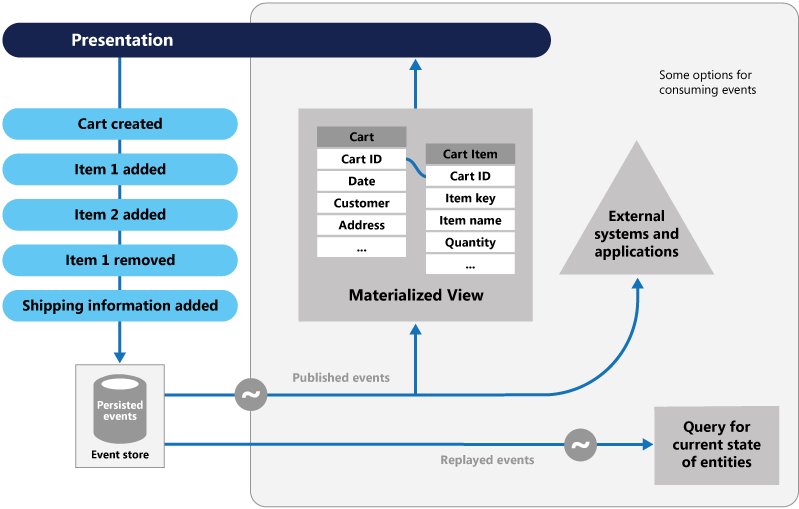
\includegraphics[width=0.70\textwidth]{myImages/event-sourcing.png}
\caption{Event Sourcing Pattern}
\label{fig:event_sourcing}
\end{figure}

Moreover, event sourcing pattern makes it possible to implement temporal queries that determine the state of an entity at any point in time.
Append-only storage mechanism enables to see the actions taken related to a particular set of data, as well as assisting in testing and debugging \cite{event_sourcing_docs}.

\subsubsection{Service Instance per Virtual Machine}
\label{subsubsec:per_vm}

The microservices architecture promotes some ideas also for the deployment stage of the software lifecycle and these ideas are, as expected, built around loose-coupling paradigm.
The first of these patterns regarding the deployment process is service instance per virtual machine (VM) pattern.
Basically, in this method, each microservice is packaged as a VM image and deployed as an application running in its own VM, possibly with other VMs running on an hypervisor-based machine which is managed by Infrastructure-as-a-Service (IaaS) provider, such as AWS EC2, Google Compute Engine and Digital Ocean.
Packaging of a service as a VM image results in ease of scaling of services, which can also be automatically done by the IaaS provider based on the load.
Moreover, the details of the implementation of the service can be encapsulated in a VM image, therefore the dependence of the service technology over the physical host can be reduced.
With regard to the drawbacks, it is time-consuming for developers to create VM images and configure infrastructure components such as load balancers and firewalls.

\subsubsection{Service Instance per Container}
\label{subsubsec:per_container}

Another microservice pattern regarding the deployment aspect is service instance per container pattern.
Similar to packaging each service as a VM image, this pattern proposes packaging each service as a container image, in most cases, as a Docker image.
According to the official docs, Docker is an open platform for developing, shipping, and running applications, and provides the ability to package and run an application in a loosely isolated environment called a container \cite{docker_def}.
Docker containers provide many of the same advantages as VM images, however, due to the underlying virtualization method, Docker containers are much more lightweight with respect to VMs \cite{eder2016hypervisor}.
Rather than using a separate operating system, containers share a operating system, resulting in a significantly smaller size of each deployment.
Underneath, Docker make use of "linux kernel namespaces" and "control groups" to isolate resources of a single virtual or physical host (a single operating system in both cases) and allows Docker containers and services inside to consume resources of the host.
Being a more "micro" approach, containers make it easier for developers to package and share an application through "Docker Hub" and deploy a service as a container image, which is built with specifications taken from a "Dockerfile", to a private cloud or a Container-as-a-Service (CaaS) provider, such as Google Cloud Run or AWS Fargate.
Moreover, the overall resiliency of the application can be improved since it takes less time and effort to run a container with respect to a service with its own operating system.
For the sake of a clear understanding of the two virtualization methods mentioned, and how they differ from traditional deployment methods, the evolution of concepts are illustrated in Figure~\ref{fig:hypervisor_vs_container}. As a side note, it is interesting to see the same evolution towards fine-granularity, seen in application architecture from monoliths and SOA to microservices, also in software deployment approaches.

\begin{figure}[H]
\centering
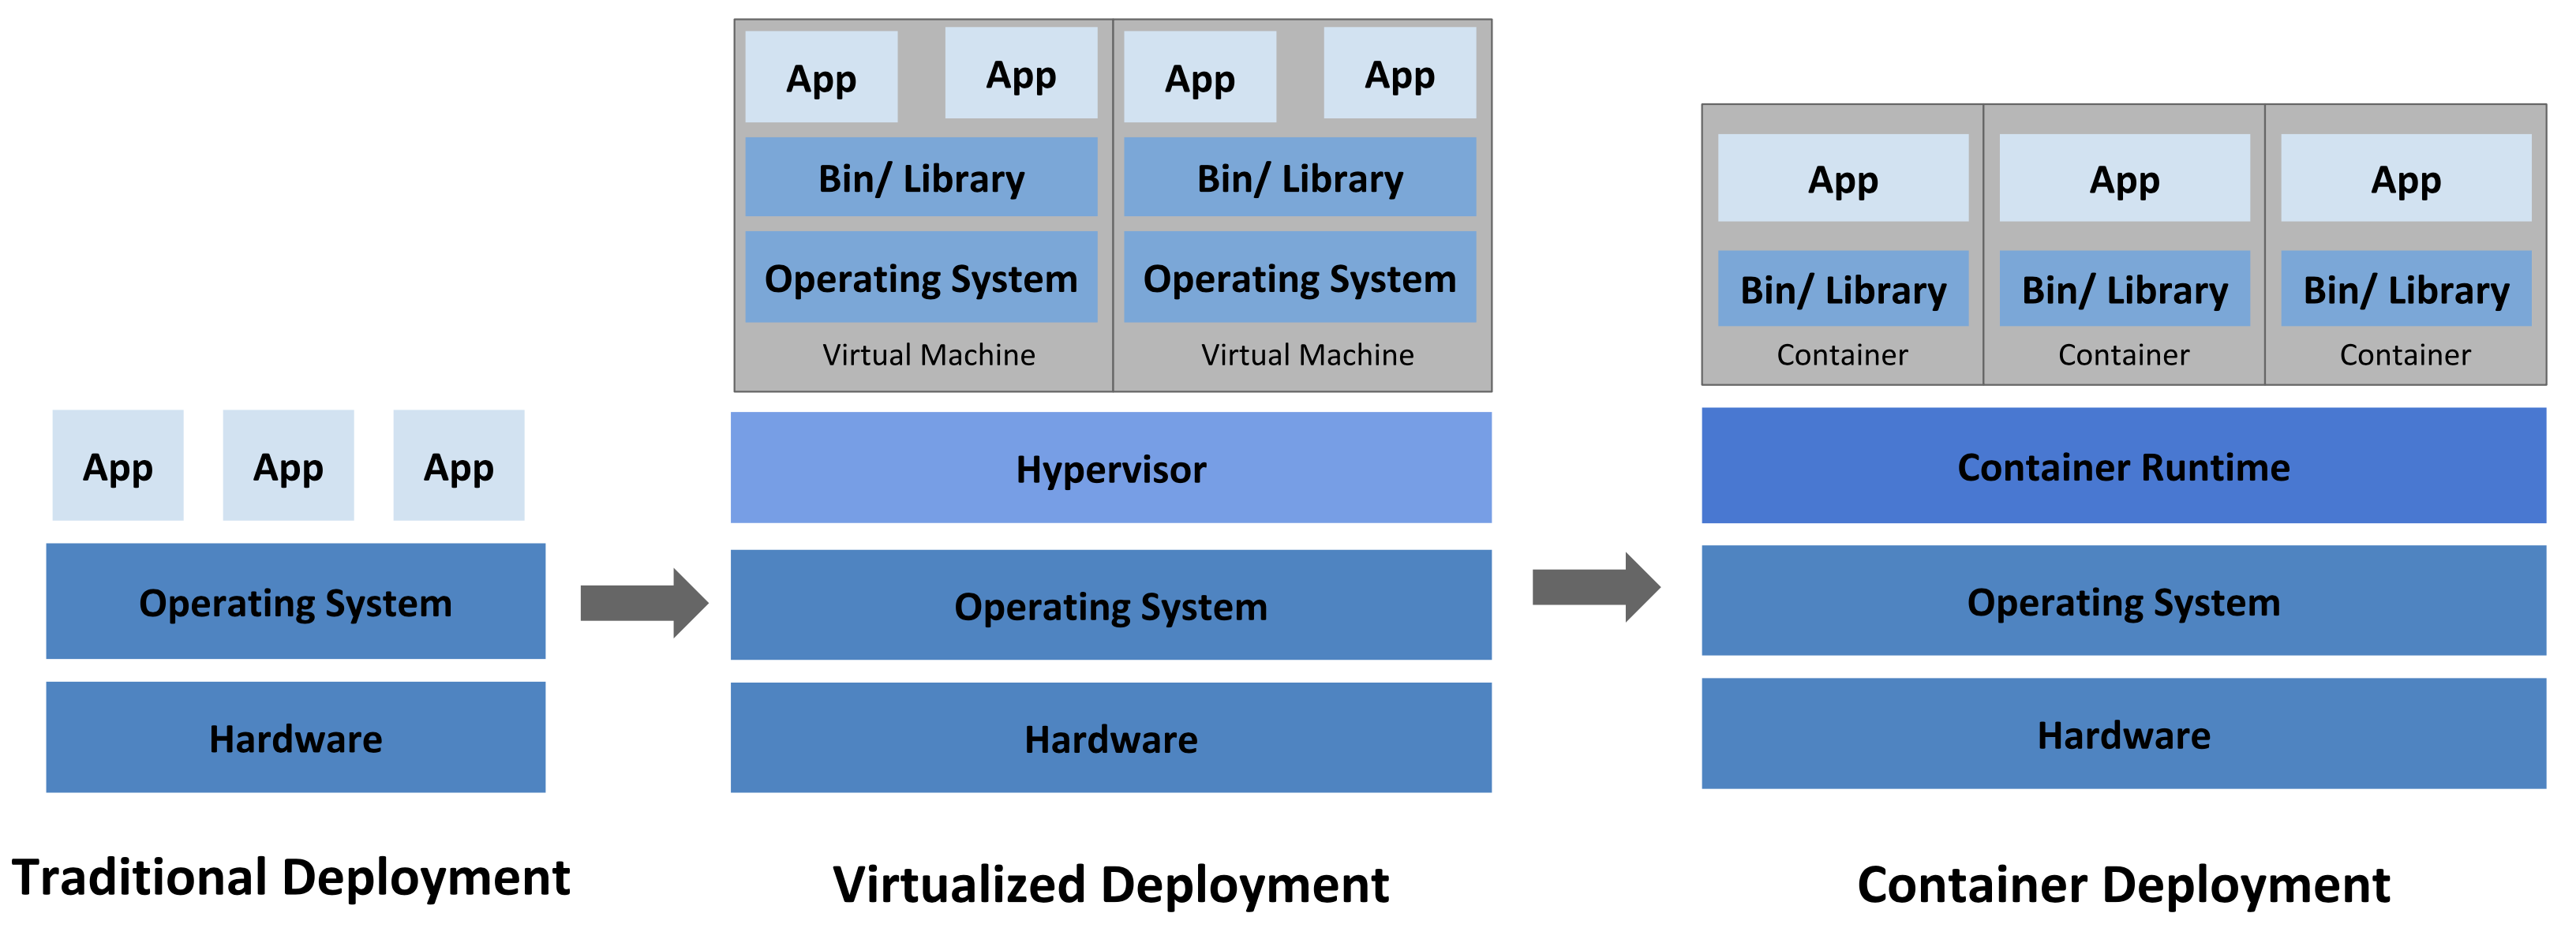
\includegraphics[width=0.90\textwidth]{myImages/kubernetes_evo.png}
\caption{Comparison and evolution of traditional, hypervisor-based and container-based deployment}
\label{fig:hypervisor_vs_container}
\end{figure}

Microservices applications consist of tens or hundreds of microservices, and considering multiple instances for some services, the total number of service instances can be quite high.
In order for the advantages promised by the microservice architecture, supposing the adoption of container-based deployment, the cluster of containers must be properly instantiated, managed and observed.
To simplify the management of a cluster of containers, there are container orchestration platforms, such as Kubernetes, AWS Elastic Container Service, Docker Swarm and Mesosphere.
Among them, Kubernetes was initially developed by Google, open-sourced in 2014 and since then has been the most widely used container orchestration platform.
At this point, to see how containerization technology and orchestration platforms comes together to realize a microservice application, it is crucial to mention some capabilities of Kubernetes and challenges it tackles.
Some of the features of Kubernetes are:
\begin{itemize}
    \item Service Discovery and Load Balancing: Kubernetes exposes container via a DNS name or IP address to the cluster, can deploy an "ingress" component that can as as an API gateway, and can distribute network traffic between service instances if the load is high.
    
    \item Storage orchestration: Allows mounting (attaching, binding) of different storage options such as local storage and public cloud provider, to the containers.
    
    \item Automated rollouts and rollbacks: Enables developers to describe the desired state of the containers at hand and via a feed-back mechanism, tries to realize the desired state into the actual state of the cluster. In other words, "rolls out" changes in a progressive way and if something bad happens, "rolls back" changes to the previous stable state. It can create or remove containers and some kinds of Kubernetes objects such "Pods", "Deployments" and "Services" to carry out the task.
    
    \item Automatic bin packing: When provided with the information of how much CPU and memory a container needs, Kubernetes can figure out how to place containers to a set of nodes so that the resources are best utilized.
    
    \item Self-healing: Restarts containers that failed, and based on user-defined health-check, replaces or kills containers that do not respond. Moreover, it routes traffic to healthy instances until the failed container is ready to handle requests.
    
    \item Secret and Configuration Management: Stores and manages sensitive information such as passwords, OAuth access token and SSH keys. Without having to re-build container images, stores and updates application configuration such as environment variables.
\end{itemize}

In addition to stand-alone Kubernetes platform for on-premise solution, the cloud providers offer Kubernetes-as-a-Service options, such as Google Kubernetes Engine (GKE), AWS EKS and Azure AKS, that enables to run Kubernetes clusters on the cloud, by means of container images and Kubernetes config files.
\\
As a consequence of the capabilities explained above, and as also stated by researchers from IBM in a research paper \cite{jaramillo2016leveraging}, it is appropriate to say that Docker has been a disruptive technology which changed the way applications are developed and distributed.
Following the same concepts and ideas as microservice architectural paradigm itself, Docker is quite a good fit for building and deploying microservices.

\subsubsection{Serverless}
\label{subsubsec:serverless}

Services as source codes can be packaged (eg, as a ZIP file) and uploaded to the deployment infrastructure, which is an utility operated by a public cloud provider.
The infrastructure hides any concept of servers, resources, virtual machines and containers, it just takes the code and runs it.
Under the hood, it uses virtual machines and containers to isolate the services.
The client (of this service) is charged for each request based on the resources consumed.
This solution is very elastic in terms of scaling, however, it comes with significant constraints in the environment.
As an example, AWS Lambda limits the maximum time it can take for a microservice to serve a request to be fifteen minutes, making it unsuitable for microservices that need to execute for longer amount of time, such as data-processing batch jobs \cite{aws_lambda}.
Another important constraint in serverless pattern is, the microservices need to be "stateless", in other words, the microservice should not assume the existence of a particular data in its local file storage or memory to serve requests, instead, the state should be stored in persistence services such as AWS S3.
Constraints such as these allow small microservices to be instantiated quickly, making it suitable for developers to deploy particular microservices that are not called frequently enough to be deployed to its own host, reducing the insfrastructure costs.
Examples include AWS Lambda, Google Cloud Functions, Azure Functions.

\subsubsection{Health Check API}
\label{subsubsec:health_check_api}

Microservices, as any other software component, can crash or fail to serve the requests even if they still run.
During the times of unavailability, it is critical to notice those services that cannot carry out requests so that the requesting services do not wait unnecessarily, and instead, if there is another healthy instance of the failing service, are routed to those available instances.
Since the scope of a microservice is in general small, the availability status in terms of sufficient disk memory, connection to a database or a cache service or in general any other service it is dependant upon, can be coded or created from features of the framework used.
As an example, the microservice can have an health check endpoint such as "/api/v1/health", and can respond to GET request with the status of the service described in a simple JSON file, possibly with HTTP status codes such as 200, 204, or 500, which stand for "OK", "No Content" and "Internal Server Error", respectively.
\\
In addition to health check mechanisms as code, the container orchestration platform Kubernetes offers health check methods that can be configured descriptively in Kubernetes configuration file by developers.
Kubernetes offers two kinds of health checking or "probing" options, named as liveness and readiness, and can carry out the health checks in periodic time intervals specified.
The first type, liveness. refers to whether a set of one or more containers, also knows as a "pod", is responsive or not.
In cases of a crash or a deadlock situation, restarting the pod can help make the service available again.
The second type, readiness, is used to decide if the service is ready to serve the requests, i.e., serves request only after loading data or configruation files or checking with services it depends on.
The health check API pattern, as seen from examples, is in fact helpful to detect and manage failures in microservices and hence the whole system, improving the resiliency of the application.

\subsubsection{Log Aggregator}
\label{subsubsec:log_aggregator}

As mentioned in the previous health check API pattern, from time to time, microservices may fail to serve the request and in some cases, it takes more than simple restarting the service to solve the issue.
Developers might need to take a look in the log files to find the exact cause of the problem.
In a microservice application, however, inspecting log files of a microservice by connecting to its host can be frustrating.
One reason is, there can be multiple instances of a microservice on different host, and it would be time-consuming to find the right host, especially if the services are scaled to new host automatically.
Another reason might be that, merely finding log files in most cases does not suffice to remove the bug, but trouble-shooting the microservices and comparing the logs from a chain of microservices is needed.
In order to ease the trouble-shooting process, log aggregator pattern can be utilized.
\\
Essentially, what log aggregator pattern proposes is, creating a central service and simply aggregating all log files from other microservices instances. Although this is simple idea, with some additions, the trouble-shooting process and developer experience can be significantly improved.
Through a configuration or log aggregator service, different logging types with various levels of detail can be specified to running microservices.
After creating a structured logging for all microservices with appropriate fields, to some extent, aggregated log files can be searchable.
Furthermore, advanced analyzing tools can be used to have more insights about the whole system.
As an example, ElasticSearch, Logstash and Kibana tools, also known as "ELK" stack, are widely used for this purpose.
From microservices themselves or from a message broker, the logs are sent to data ingestion tool Logstash, and afterwards, ElasticSearch is used to analyze text or JSON data and Kibana is used to visualize the results to make the data more presentable for developers and data analysts.
Another example from a public cloud provider is AWS CloudWatch.
In addition to above-mentioned capabilities of ELK stack, CloudWatch can be configured to send alerting events or do some operational changes such as auto-scaling, if a particular word or a message occurs among the logs.

\subsubsection{Distributed Tracing}
\label{subsubsec:distributed_tracing}

In a microservice architected application, in contrary to a monolithic application, a request does not get handled by a single software component but rather by multiple microservices needed for that particular request.
From a system-wide point of view, a request, whether it is from an external UI agent or an internal microservice for a background job, results in an execution of a chain of microservices.
Naturally, this type of multi-call mechanism of microservices brings about complexity in terms of application development and performance monitoring.
For example, it would be helpful for developers to see which microservices are being called and which bounded domain contexts are being touched by a specific request.
Another exemplary scenario is that, some microservices might take more time to execute their tasks before calling the next microservice in the chain, so it would be beneficial to acquire how long it takes for microservices to complete their tasks so that the bottleneck of the system can be pinpointed and improved.
For these kind of tasks, distributed tracing pattern can be quite advantageous.
\\
In essence, distributed tracing pattern suggests assigning IDs to each external requests and passing it along with each call down the chain or path of execution, so that the path can be traced.
Each microservice is attached or instrumented with an agent that creates new spans for incoming requests and attaches context information required for identification to outgoing request.
Similar to log aggregator pattern, a central collector service reveices trace data from agents, validates and stores data to be queried.
Finally, a query process queries the tracing database and shows the result of the query, possibly as a visualization using nodes, arrows or nested spans and related data.
Figure~\ref{fig:jaeger_trace} illustrates a detailed view of inter-service calls resulted from a GET request to an endpoint in frontend service, created by Jaeger, which is an open-source distributed tracing system.

\begin{figure}[H]
\centering
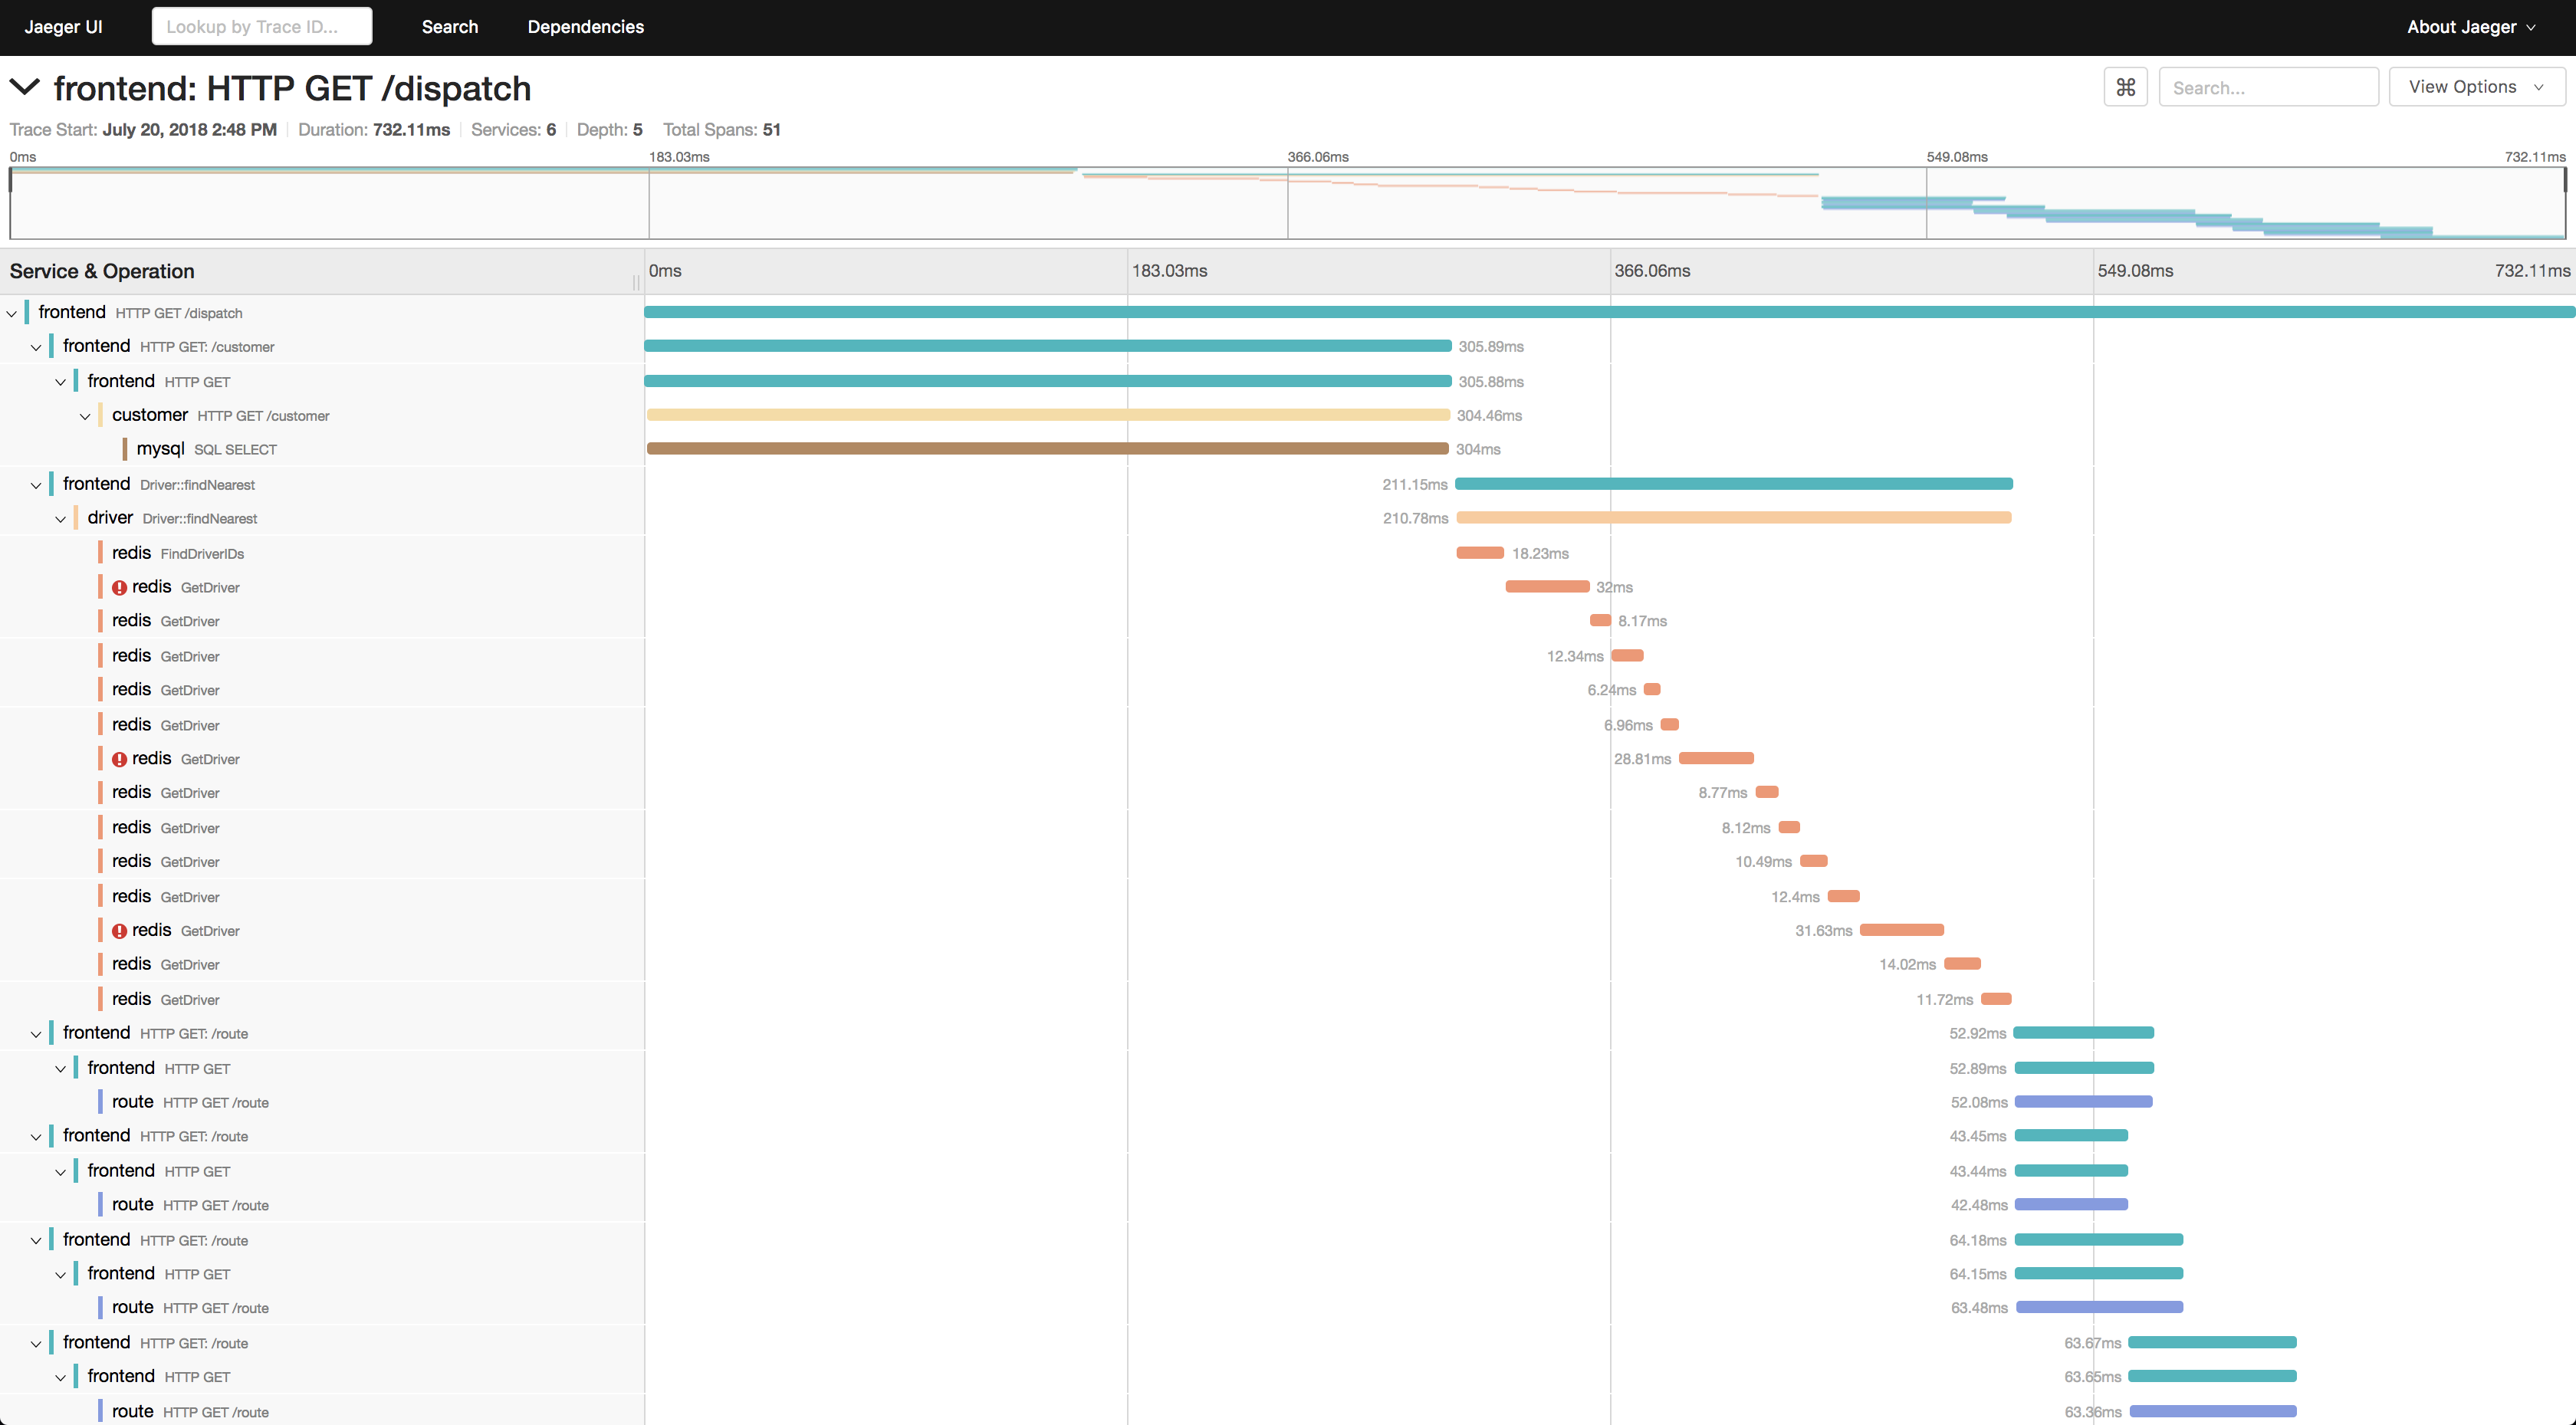
\includegraphics[width=1.0\textwidth]{myImages/trace-detail-ss.png}
\caption{Visualization of inter-service calls and timing data by Jaeger}
\label{fig:jaeger_trace}
\end{figure}

As mentioned above, the distributed tracing pattern, similar to a service mesh, can be divided into two parts, an intrumentation or tracing part and the collection part.
Unsurprisingly, in order for a system to have distributed tracing capability, these two parts must be compatible, in other words, they must adhere to the same API specification.
In the open-source community, although there is no standardization yet, collective efforts such as OpenTracing tries to create a standardization of APIs, naming of concepts and shows tools such as Jaeger that complies with the OpenTracing standard.
Another major distributed tracing system Zipkin, which supports distributed tracing integration with popular cloud frameworks such as Spring Cloud.

\subsection{Anti-Patterns}
\label{subsec:antipattern}

\subsubsection{Wrong Cut}
\label{subsubsec:wrong_cut}

As mentioned previously, microservices are designed using bounded context method, that is, each microservice is designed to carry out tasks related to one small business capability.
One misconception for the separation of microservices is the construction of microservices in a layered fashion, as opposed to having one business capability.
Designing microservices so that each microservice takes care of a major task from a technical perspective of the whole application is in fact a bad habit from SOA.
To explain shortly and to not repeat the differences between SOA and microservices architectures, it is appropriate to say that, while designing microservices in a layered style like UI, logic and data increases re-usability of both code and data, it conflicts with the requirements needed for the microservice architecture to deliver its benefits.
The wrong cut anti-pattern causes deployments to be dependant on other services, breaks team independence and brings about high-coupling, since each business task would then require more microservices to be available.
To avoid this pattern, microservices should be designed from a business perspective and the ownership of logic and data to a development team should be preserved.

\subsubsection{Cyclic Dependencies}
\label{subsubsec:cyclic_dependencies}

An application that employs the microservice architecture style handles external request through a chain or path of microservice calls.
For that reason, during run-time, the whole application can be visualised as a directed graph, specifically, microservices as nodes and calls as arrows.
The cyclic dependencies anti-pattern is, basically, a cyclic span of connected arrows on the graph, implying that, there is, or can be, a request that might result in microservices calling each other in a cyclic order.
Due to a bug in code, or a bad decision during the design phase, a particular request can cause microservices that take part in the cyclic service calls, to call each other indefinitely.
Even if the cyclic call ends by design, it is a sign of high coupling between microservices, hinting at the possibility that, the microservices might have designed so small that they cannot carry out business capabilities without being dependant on each other's logic or data.
To remedy this anti-pattern, the microservices that appear in the cycle can be re-designed and perhaps merged into a single microservice, yet taking into consideration that the new microservice does not become a megaservice.

\subsubsection{}
\label{subsubsec:wrong_cut}

\chapter{Adopted Methodology}
\label{ch:method}%

\section{Classification of Patterns}
\label{sec:class_method}

\section{Selection of Open Source Projects}
\label{sec:select_method}

\section{Detection of Patterns}
\label{sec:detection_method}

\chapter{Results}
\label{ch:results}%

\section{Resulting Classification of Patterns}
\label{sec:class_result}

\section{Selected Open Source Projects}
\label{sec:select_result}

\section{Detected Patterns in Selected Projects}
\label{sec:detection_result}

\section{Discussion of Findings}
\label{sec:discussion}

\chapter{Conclusion}
\label{ch:conclusion}%

%-------------------------------------------------------------------------
%	BIBLIOGRAPHY
%-------------------------------------------------------------------------

\addtocontents{toc}{\vspace{2em}} % Add a gap in the Contents, for aesthetics
\bibliography{myThesisBib}

%-------------------------------------------------------------------------
%	APPENDICES
%-------------------------------------------------------------------------

\cleardoublepage
\addtocontents{toc}{\vspace{2em}} % Add a gap in the Contents, for aesthetics
\appendix
\chapter{Appendix A}
If you need to include an appendix to support the research in your thesis, you can place it at the end of the manuscript.
An appendix contains supplementary material (figures, tables, data, codes, mathematical proofs, surveys, \dots)
which supplement the main results contained in the previous chapters.

% LIST OF FIGURES
\listoffigures

% LIST OF TABLES
\listoftables

% LIST OF ABBREVIATIONS
% Write out the List of Symbols in this page
\chapter*{List of Abbreviations}
\begin{table}[H]
    \centering
    \begin{tabular}{ll}
        \textbf{Abbreviation} & \textbf{Description} \\\hline\\[-9px]
        AMQP & Advanced Messaging Queuing Protocol \\[2px]
        API & Application Programming Interface \\[2px]
        BC & Bounded Context \\[2px]
        CI/CD & Continuous Integration / Continuous Delivery \\[2px]
        CaaS & Container-as-a-Service \\[2px]
        CQRS & Command Query Responsibility Segregation \\[2px]
        DDD & Domain Driven Design \\[2px]
        ESB & Enterprise Service Bus \\[2px]
        HTTP & Hypertext Transfer Protocol \\[2px]
        IaaS & Infrastructure-as-a-Service \\[2px]
        JSON & Javascript Object Notation \\[2px]
        LOC & Lines of Code \\[2px]
        MSMQ & Microsoft Messaging Queuing \\[2px]
        NoSQL & Not-Only-SQL, to refer to different kinds of non-relational databases \\[2px]
        QoS & Quality of Service \\[2px]
        REST & Representational State Transfer \\[2px]
        RESTful API & an API that adheres to REST principles \\[2px]
        SOA & Service Oriented Architecture \\[2px]
        SOAP & Simple Object Access Protocol \\[2px]
        SQL & Structured Query Language \\[2px]
        SSH & Secure Shell \\[2px]
        TLS & Transport Layer Security \\[2px]
        UI & User Interface \\[2px]
        UX & User Experience \\[2px]
        VM & Virtual Machine \\[2px]
    \end{tabular}
\end{table}

% ACKNOWLEDGEMENTS
\chapter*{Acknowledgements}
Here you might want to acknowledge someone.

\cleardoublepage

\end{document}
